\section{Implementation}
\label{s:implementation}
\hspace{10pt} In this section, the implementations of the the software components and the experiments involved in the dissertation are discussed. The design presented in the previous section is revisited. The first subsection summarizes the problems occurred while comparing sensors' energy profiles. It describes the issues related to Android operating system, differences between mobile devices, failed samples in the experiment and Android API. The second subsection presents the implementation details of the energy efficient sensing library, Sensy. [XXX keep going here on Sensy + rewrite next sentence]. The implementation process results in new knowledge on energy-accuracy of phone sensing, which is summarized in the last subsection.

\subsection{Sensors energy measurements}
intro:\\
	how did i end up doing it/problems\\
	generally: available phones + android versions, how old they were, specifications(sensors)\\
		table!\\
	
\begin{center}
    \begin{tabular}{| l | c | c | c |}
    \hline
      & Google Nexus 7 & HTC Flyer & HTC desire \\ \hline
    Android version & 4.3 & 3.3 &  2.3.3\\ \hline
    Battery & X & X & X\\ \hline
    Camera & \checkmark & \checkmark & \checkmark\\ \hline
    Microphone & \checkmark & \checkmark & \checkmark \\ \hline
    IEEE 802.11 & \checkmark & \checkmark & \checkmark \\ \hline
    GPS & \checkmark & \checkmark & \checkmark \\ \hline
    Bluetooth & \checkmark & \checkmark & \checkmark\\ \hline
    Bluetooth LTE & \checkmark & - & - \\ \hline
    Accelerometer & \checkmark & \checkmark & \checkmark\\ \hline
    Gyroscope & \checkmark & - & -\\ \hline
    Magnetic Field & \checkmark & \checkmark & \checkmark\\ \hline
    Ambient Light & \checkmark & \checkmark & \checkmark\\ \hline
    Proximity & - & -& \checkmark\\ \hline
    \end{tabular}
\end{center}		
	
\subsubsection{Android operating system}
problem: slow battery depletion\\
	solution: screen on for all apps\\
		increase battery consumption\\
	result: comparison\\

problem: Wireless\\
	switching off WiFi on Android phones\\
		Android switches wireless on from time to time -> special option for those \\
		
	active/passive sampling\\
		why Google doesn't do active scanning?!
			advanatages: faster
			disadvanatages: 
				-energy:
					"radio modem transmission typically requires about 10 times as much power as reception"
				-AP will only respond if i probe direct 
				-introduce additional  traffic
				-privacy:
					Presence analytics\\
						cisco tristan twitter\\
							around time of chickenpox doughter\\
							https://meraki.cisco.com/lib/pdf/meraki\_whitepaper\_presence.pdf\\
				
				
	caching Wireless results\\
		-move around check whether it changes
			-are results the same?
		checked with Kismac

\subsubsection{Differences between mobile phones}
problem: different percentage for different phones\\
	end up checking different ones for different phones\\
		trace what I checked for each\\
		HTC Flyer\\
			charging battery to 100\% took forever\\
			then, battery depletion from 100\% to 99\% takes forever\\
			very very fast depletion from 99\% to 95\%\\
		HTC Desire\\
			choose 89->88, as it is old phone and charging was not triggered till if battery level more than 91\%\\
		
problem: hardware differences between phones\\
	camera:\\
		not enough dynamic memory on HTC desire -> but standardize codecs/size to fit all\\
		-Google Nexus 7, HTC desire, HTC flyer:\\
					-Codec H263\\
					-Resolution	176\&144\\
					-Frame rate		~10(HTC flyer),	~12(HTC desire),	~15(Google Nexus 7)\\
		audio saving -> memory issues\\
			codex issues then\\
	microphone:\\
		(standarized as much as possible)
		Google Nexus 7:\\
			-Codec: AMR narrow band(samr)\\
			-channels: 		mono\\
			-sample rate:	8000 Hz\\
			-bits per sample 	32\\
		HTC desire, HTC flyer:\\
			-Codec: AMR narrow band(samr)\\
			-channels:		1\\
			-sample rate:	8000 Hz\\
			-bits per sample:	16\\
			-Bitrate:		128 kb/s	\\
			
\subsubsection{Failed samples}
problem: failed samples\\
	table with failed samples\\
	Google Nexus 7 nice:\\
		results are stable, but others not really\\
			-> so up to 5 successful samples for other phones\\
	reasons why invalid\\
	
	also, battery seems to be getting less stable
	
	Google Nexus 7\\
\begin{table}
    \begin{tabular}{| l | c | c | c |}
    \hline
    Plain                  & 902 & 902 & 841 \\ \hline
    Ambient Light          & 841 & 902 & 841\\ \hline
    Bluetooth Low Energy*  & 782 & 842 & 781 \\ \hline
    Magnetic field:        & 782 & 782 & 721\\ \hline
    Microphone             & 721 & 781 & 782 \\ \hline
    Bluetooth classic      & 781 & 721 & 722 \\ \hline
    Accelerometer:         & 781 & 721 & 661 \\ \hline
    Gyroscope              & 721 & 722 & 721 \\ \hline
    Bluetooth Low Energy** & 722 & 721 & 661 \\ \hline
    \end{tabular}
\end{table}


   HTC Flyer\\
\begin{table}
    \begin{tabular}{| l | c | c | c | c | c | c | c | c | c |}
    \hline
    Plain          & \cellcolor{red!25}30  & 270  & 270   & 270   & 271       & 270 & 270      & ~   & ~   \\ \hline
    Bluetooth      & 181\^ & 270  & \cellcolor{red!25}30   & \cellcolor{red!25}60   & 270       & 271 & 270      & 241 & 264 \\ \hline
    Accelerometer  & 240  & 270  & 180\^ & 271   & 240       & 270 & 258      & ~   & ~   \\ \hline
    Magnetic field & 270  & 180\^ & 240   & \cellcolor{red!25}30   & 300^^   & 240 & 270      & 270 & 258 \\ \hline
    Light          & 240  & 240  & 271   & 270   & 270       & 258 & ~        & ~   & ~   \\ \hline
    Microphone     & 240  & 240  & 240   & 300^^ & 270       & 240 & 246      & ~   & ~   \\ \hline
    WiFiScan       & 240  & 241  & 236   & 248   & 240(HOME) & 240 & 240      & ~   & ~   \\ \hline
    GPS            & 241  & 240  & 210   & \cellcolor{red!25}30   & 120^^   & 240 & 240(OUT) & 210 & 228 \\ \hline
    Camera         & 121\^ & 240  & 180^^ & 210   & 241       & 240 & 210      & 228 & ~   \\ \hline
    \end{tabular}
\end{table}

	HTC Desire\\
	\begin{table}
    \begin{tabular}{| l | c | c | c | c | c | c | c | c | c | c | c | c |}
    \hline
    Plain          & 250  & 253  & 251  & 201  & 250  & 240          & ~     & ~   & ~    & ~    & ~   & ~   \\\hline
    Bluetooth      & 251  & 251  & 200  & 250  & 250  & 240          & ~     & ~   & ~    & ~    & ~   & ~   \\\hline
    Light Sensor** & 251  & 251  & 251  & 200  & 451\^ & 451\^        & 200   & 230 & ~    & ~    & ~   & ~   \\ \hline
    Proximity*     & 251  & 501\^ & 451\^ & 200  & 501\^ & 463\^        & 251** & 251 & 403\^ & 401\^ & 200 & 230 \\ \hline
    Accelerometer  & 251  & 451\^ & 200  & 401\^ & 200  & 250          & 250   & 230 & ~    & ~    & ~   & ~   \\ \hline
    Magnetic Field & 201  & 250  & 201  & 400\^ & 200  & 253          & 220   & ~   & ~    & ~    & ~   & ~   \\ \hline
    Microphone     & 400\^ & 200  & 200  & 250  & 200  & 450\^        & 250   & 220 & ~    & ~    & ~   & ~   \\ \hline
    WifiScan       & 150  & 300\^ & 251  & 201  & 250  & 251(LIBRARY) & 151   & 200 & ~    & ~    & ~   & ~   \\ \hline
    Camera         & 150  & 200  & 201  & 200  & 200  & 190          & ~     & ~   & ~    & ~    & ~   & ~   \\ \hline
    GPS            & 200  & 201  & 150  & 200  & 151  & 170          & ~     & ~   & ~    & ~    & ~   & ~   \\ \hline
    Light Sensor*  & 501\^ & 451\^ & 501\^ & 451\^ & 502\^ & 480          & ~     & ~   & ~    & ~    & ~   & ~   \\ \hline
    \end{tabular}
\end{table}

\begin{figure}[H]
\centering
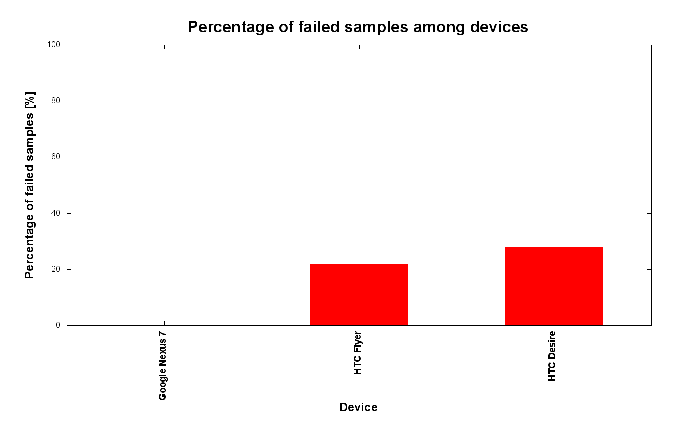
\includegraphics[scale=1.5]{plots/devices_failed_samples.eps}
\caption{Percentage of failed samples among devices }
\end{figure}


\begin{figure}[H]
\centering
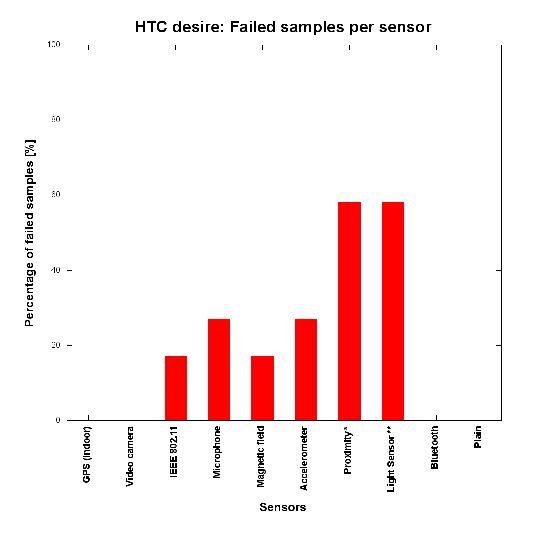
\includegraphics[scale=1.5]{plots/htc_desire_failed_samples.eps}
\caption{HTC Desire: Failed samples per sensor }
\end{figure}

	Trepn Profiler\\
	
	
	
	Calibration of results mention here!\\

\subsubsection{Android API}
smaller issues(API and energy efficiency?):\\
	Bluetooth Low Energy\\
		new in Android 18\\
		shaky(no callback when finished):
			-when devices visible ->prints a lot of logs) -> higher energy consumption\\
			-no devices available is good
		
	Camera needs to have a preview\\
		so uses more energy\\
   
   switching off WiFi in Android:\\
   		Google Location Service\\
   
\subsubsection{Conclusions}   
conclusion: on the whole method\\
	accurate\\
	instability of battery\\
		many invalid samples, bursty errors\\
	not universal solution\\
		different percentages work across devices\\
	all of theses makes a method impractical, as requires many samples to get accurate result
		-can't be used as online measurement tool\\

\subsection{Sensy}
\subsection{Conclusions}